\newpage
\section{A complete projection example}
To obtain the position of the pixels on screen from the local coordinates that define the 3D model five steps should be performed:
\begin{enumerate}
\item World Transform
\item View Transform
\item Projection
\item Normalization
\item Screen Transform
\end{enumerate}
Each steps performs a coordinate transformation from on 3D space to another.
The first three can be done with a \textbf{matrix-vector} product.
The screen transform can be done possibly also this way. Normalization instead requires a different procedure.

\subsection{World-View-Projection Matrices}
\begin{description}
\item[1. Model]\hfill\\
 Firstly a 3D model is created in local coordinates $p_M$. Local coordinates are usually 3D Cartesian coordinates and are firs transformed into\textbf{ homogeneous coordinates} $p_L$ by adding a \textbf{forth} component equal to 1.\\
 $$ p_M = |p_{Mx} \quad p_{My} \quad p_{Mz}|$$
 $$p_L = = |p_{Mx} \quad p_{My} \quad p_{Mz} \quad 1|$$
\item [2. World Matrix]\hfill\\
The \textbf{World Transform} converts the coordinates from local space to global space by multiplying them by the \textbf{World Matrix} : 
$$ p_W = M_w \cdot p_L$$
\item[3.View Matrix]\hfill\\
The view transform allow to see the 3D world from a given point in space.It transforms the global space coordinates into \textbf{camera space coordinates} by using the \textbf{View Matrix} $$ p_V = M_V \cdot p_W$$.
\item[4.Projection Matrix]\hfill\\
The projection transformation prepares the coordinates to be shown on screen by performing either a \textbf{parallel} or \textbf{perspective} projection.\\
For parallel projections the transformations is performed using a parallel projection matrix $M_{P-ort}$ and it converts the camera space coordinates into \textbf{Normalized Screen Coordinates}\\
For perspective projections the transformations is done using a perspective projection matrix $M_{P-pers}$ and it converts the camera space coordinates into \textbf{Clipping Coordinates} (! not \textbf{normalized}!)
$$ p_C = M_p \cdot p_V$$
\end{description}
These matrices can be compressed in a single matrix (\textbf{World View Projection Matrix}) : $$ p_C = M_p \cdot M_V \cdot M_W \cdot p_L = M_{WVP} \cdot p_L$$

The \textbf{Normalization } step is require in case of perspective projections where the transformations produces \textbf{clipping coordinates}. As opposed  to other transformations this step is done by normalizing the homogeneous coordinates that describe the points  in the clipping space. Every component is divided by the fourth component and the last component is then discarded :
$$ |x_C \quad y_C \quad z_C \quad w_C| \to \left | \frac{x_C}{w_C} \quad \frac{y_C}{w_C} \quad \frac{z_C}{w_C} \quad 1 \right | \to (x_N,y_N,z_N)$$
This must be done only for perspective projections as the parallel ones already result in normalized coordinates where it is sufficient to just drop the last component.\\
This normalization step is performed by the video cart adapter and is transparent to the user : it first transforms the clipping coordinates in normalized screen coordinates and the into pixel coordinates to show objects
$$ (x_S,y_S) = \left ( \frac{S_W-1}{2} \cdot(1+x_n) , \frac{S_h-1}{2} \cdot(1-y_n) \right )$$
\begin{figure}[H]
  \centering
  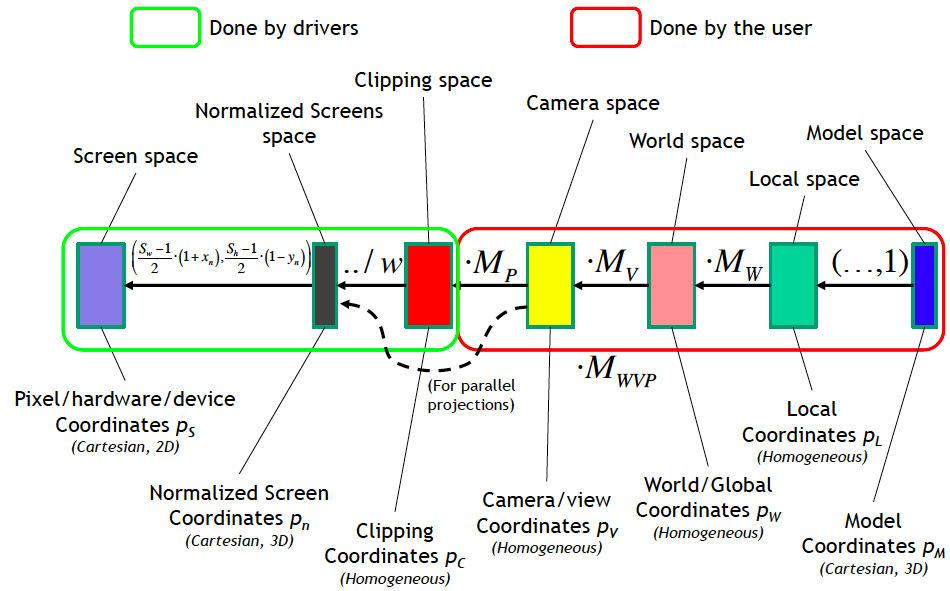
\includegraphics[width=.8\linewidth]{recap}
\end{figure}

\subsection{The example}
The starship is models with a tetrahedron and has the following local coordinates.
\begin{figure}[H]
  \centering
  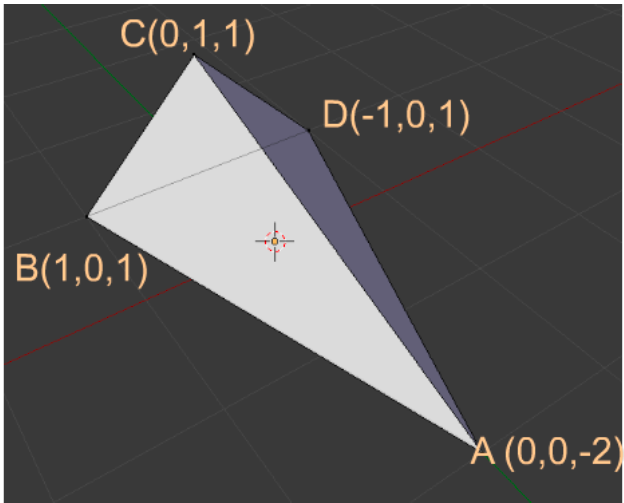
\includegraphics[width=.4\linewidth]{starship}
\end{figure}
It is facing the \textbf{negative z-axis}.\newpage
In a moment of the game the player is in position $(0,3,0)$ with
Pitch $\ang{-30}$,
Roll $\ang{0}$,
Yaw $\ang{-45}$\\
The enemy ship is in position $E(3,-1,-5)$ with
Pitch $\ang{45}$,
Roll $\ang{0}$,
Yaw $\ang{120}$
\begin{figure}[H]
  \centering
  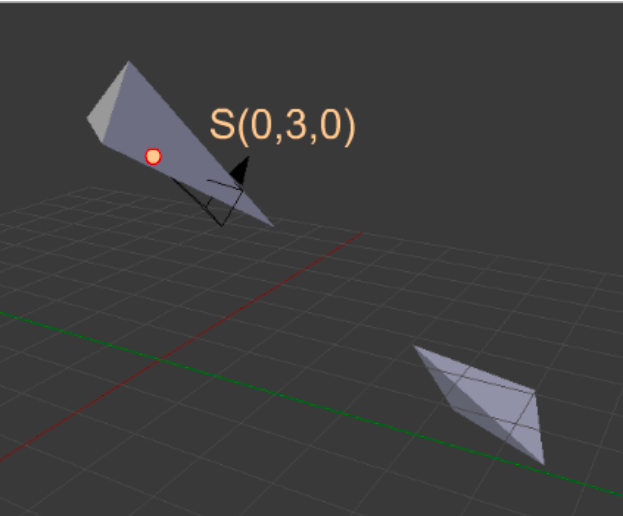
\includegraphics[width=.4\linewidth]{starship1}
\end{figure}
What are the pixel coordinates of the vertex of the tetrahedron seen on  a 960x540 pixel screen (5:4 aspect ration with non square pixels)?\\
Additional informations : 
\begin{itemize}
\item Field of View : $\ang{90}$ so quite wide-angle.
\item Near plane = 0.5 (you see windscreen of starship), far plane = 9.5 (see nothing beyond)
\item Scaling $S=(1,1,1)$
\end{itemize} 
\begin{description}
\item[World Matrix of enemy ship]\hfill\\
\begin{itemize}
\item Position $(p_x,p_y,p_z) = (3,-1,-5)$
\item Rotation Yaw,Pitch,Roll= $(\ang{120},\ang{45},\ang{0})$
\item Scaling $S=(1,1,1)$
\end{itemize}
\begin{figure}[H]
  \centering
  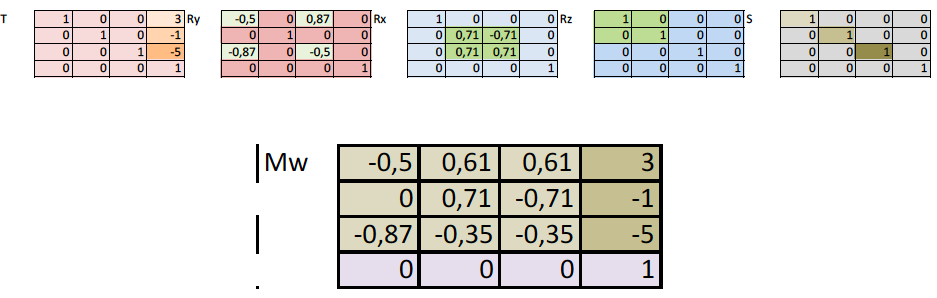
\includegraphics[width=.6\linewidth]{starshipwm}
\end{figure}
\item[View Matrix]\hfill\\
\begin{itemize}
\item Center position $(c_x,c_y,c_z) = (0,3,0)$
\item Angles $(\alpha,\beta,\rho) = (\ang{-45}, \ang{-30}, \ang{0})$
\end{itemize}
\begin{figure}[H]
  \centering
  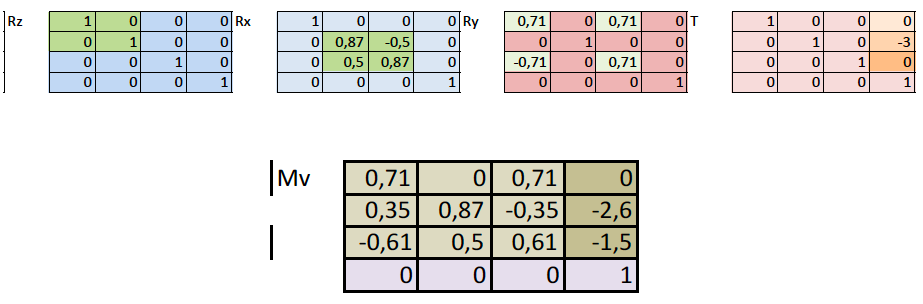
\includegraphics[width=.6\linewidth]{starshipvm}
\end{figure}
\item[Projection matrix]\hfill\\
\begin{itemize}
\item (FoV,aspect ratio) = $(90,1.25)$
\item (n,f) = $(0.5,9.5)$
\begin{figure}[H]
  \centering
  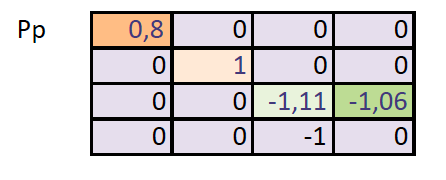
\includegraphics[width=.4\linewidth]{starshippm}
\end{figure}
\end{itemize}
\item[WVP Matrix]\hfill\\
\begin{figure}[H]
  \centering
  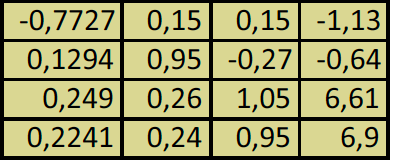
\includegraphics[width=.4\linewidth]{starshipwvpm}
\end{figure}
\end{description}
Then we multiply the points of the vertexes (to which a fourth component equal to 1 is added) with the WVP Matrix.
\begin{figure}[H]
  \centering
  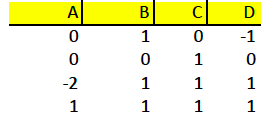
\includegraphics[width=.4\linewidth]{starshipvertexes}
\end{figure}
We obtain the \textbf{clipping coordinates}:
\begin{figure}[H]
  \centering
  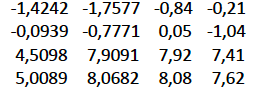
\includegraphics[width=.4\linewidth]{starshipclipping}
\end{figure}
These coordinates are then normalized (in 3D) and then transformed into 2D pixel coordinates $(343,264) , (375,244),  (430,271) , (466,233)$

\begin{figure}[H]
  \centering
  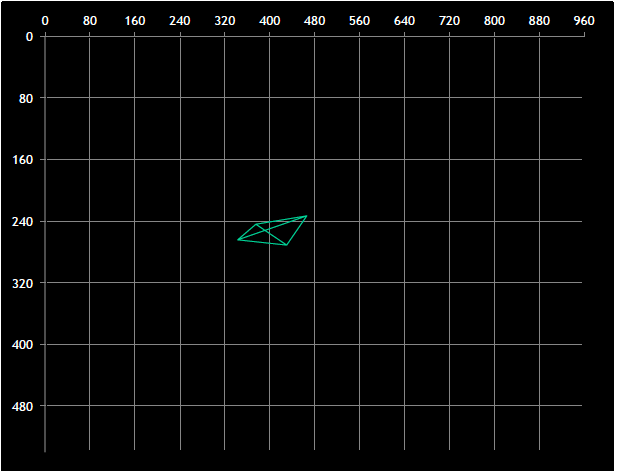
\includegraphics[width=.4\linewidth]{starshipend}
\end{figure}
